
\documentclass[a4paper,12pt]{article}
\usepackage[utf8]{inputenc}
\usepackage[polish]{babel}
\usepackage{geometry}
\usepackage{array}
\usepackage{titling}
\usepackage{setspace}
\usepackage{parskip}
\usepackage{amsmath}
\usepackage{float}
\usepackage{subcaption}
\usepackage{graphicx}
\usepackage[T1]{fontenc}
\usepackage[colorlinks=true, allcolors=blue]{hyperref}

\geometry{margin=2.5cm}
\setstretch{1.3}
\pagenumbering{style}



\begin{document}

\begin{titlepage}
\vspace{2cm}

\begin{flushright}
    \Large Marek Pąśko\\
    \Large 333352\\
    \Large Grupa: 5 - środa 14:15 - 16:00\\
    \Large Prowadzący: M.Figat\\
\end{flushright}

\vfill

\begin{center}
    \fontsize{50}{10}\selectfont
    \textbf{PROJEKT 5}\\[0.5cm]
    \textbf{Usterzenie poziome - stateczność i sterowność}\\[0.5cm]
\end{center}

\vfill

\begin{flushleft}
    \Large Data oddania projektu: 11.03.2026
\end{flushleft}

\begin{flushright}
   \LARGE Ocena: ......
\end{flushright}



\end{titlepage}
\newpage
%%%%%%%%%%%%%%%%%%%%%%%%%%%%%%%%%%%%%%%%%%%%%%%%%%%%%%%%%%%%%%%%%%%%%%%%%%

%\tableofcontents %to spis treści
%\newpage %to nowa strona

\section{Wstęp}
Niniejsze ćwiczenie polega na wyznaczeniu przebiegów przyspieszeń oraz położeń układu o dwóch stopniach swobody na podstawie danych z czujników przyspieszenia i położenia. Obiektem badanym jest wahadło umocowane za pomocą przegubu Cardana (Rysunek 1). Do pomiaru wychyleń kątowych wykorzystywane są potencjometry, natomiast do pomiaru przyśpieszeń używa się akcelerometru umieszczonego na końcu drążka.

Wyznaczenie współrzędnych ruchu układów mechanicznych na podstawie danych z czujników ma wiele zastosowań w robotyce, między innymi w systemach odometrii używanych na przykład w robotach mobilnych. Ćwiczenie pozwala również zaobserwować błędy wynikające z użytej metody pomiarowej oraz całkowania numerycznego.

\begin{figure}[H]
\centering
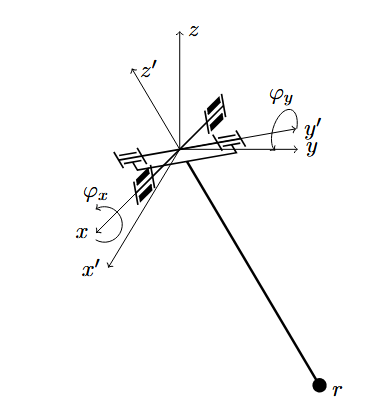
\includegraphics[width=0.7\linewidth]{Plot/uklad_pomiarowy.png}
\caption{Schemat kinematyczny wahadła}
\end{figure}

\newpage


\section{Skalowanie przyrządów pomiarowych}

Czujniki zbierają dane wyrażone w postaci napięć. Należy więc je przeskalować do odpowiedniej wielkości miary położenia oraz przyspieszenia.

\subsection{Skalowanie potencjometrów}
Dla każdego potencjometru zmierzono napięcie wyjściowe w położeniach wahadła:
$-30^\circ,\; 0^\circ, \;  +30^\circ$, a następnie policzono z nich odpowiednie współczynniki nachyleń potencjometrów:
\[
C_x = \frac{\pi/3}{U_{x}^{+30^\circ} - U_{x}^{-30^\circ}}, \qquad
C_y = \frac{\pi/3}{U_{y}^{+30^\circ} - U_{y}^{-30^\circ}}.
\]
Wyniki umieszczono w tabeli (Tabela 1).

\begin{table}[h]
\centering
\begin{tabular}{|c|c|c|}
\hline
 & Kanał $x$ & Kanał $y$ \\ \hline
$U_{\bullet}^{0^{\circ}}$ & 1,51 V & 3,54 V \\ \hline
$U_{\bullet}^{-30^{\circ}}$ & 0,83 V & 2,95 V \\ \hline
$U_{\bullet}^{+30^{\circ}}$ & 2,21 V & 4,11 V \\ \hline
$C_{\bullet}$ & 0,748 rad/V & 0,902 rad/V \\ \hline
\end{tabular}
\caption{Skalowanie potencjometrów}
\end{table}


Wartości wychyleń kątowych liczone są jako:
\[
\tilde{\varphi}_x = C_x \left( U_{x} - U_{x}^{0^\circ} \right), \qquad
\tilde{\varphi}_y = C_y \left( U_{y} - U_{y}^{0^\circ} \right).
\]

\subsection{Skalowanie akcelerometrów}

\subsubsection{Metoda $\pm 1g$}
Akcelerometr jest zdemontowany z końcówki wahadła, a kolejne jego osie ustawiane są równolegle do wektora grawitacji (raz piosono w dół, a raz w górę). Zmierzone w ten sposób napięcie zestawiono w tabeli (Tabela 2).

Następnie współczynniki nachyleń charakterystyk obliczane są według wzoru:
\[
D_x = \frac{2g}{V_{x}^{+1g} - V_{x}^{-1g}}, \qquad
D_y = \frac{2g}{V_{y}^{+1g} - V_{y}^{-1g}}, \qquad
D_z = \frac{2g}{V_{z}^{+1g} - V_{z}^{-1g}}.
\]\

\begin{table}[h]
\centering
\begin{tabular}{|c|c|c|c|}
\hline
 & Kanał $x$ & Kanał $y$ & Kanał $z$ \\ \hline
$V_{\bullet}^{0g}$ & 1,26 V & 1,26 V & 1,27 V \\ \hline
$V_{\bullet}^{-1g}$ & 1,06 V & 1,06 V & 1,04 V \\ \hline
$V_{\bullet}^{+1g}$ & 1,47 V & 1,47 V & 1,47 V \\ \hline
$D_{\bullet}$ & 47,854 $\frac{m}{s^2}/V$ & 47,854 $\frac{m}{s^2}/V$ & 45,628 $\frac{m}{s^2}/V$ \\ \hline
\end{tabular}
\caption{Skalowanie akcelerometrów metodą $\pm 1g$}
\end{table}


\newpage
\end{document}